\chapter{The ImageJ Macro Language}

When talking about programming languages it is useful to make a distinction between the syntax of the language and its semantics. In a natural language the syntax defines which combinations of symbols form a well-formed sentence. Semantics connects the words of a well formed sentence to objects and concepts of the real world or of our imagination. In other words the syntax is about the form of sentences and the semantics about the meaning.  

Likewise for computer languages the syntax defines what a well formed program in the language is while the semantics describes the behaviour of the computer when the program is executed. The behaviour can be described in terms of input, inner state of the machine and output \cite{slonneger_formal_1995}. 

We will not give a formal definition of the syntax of the ImageJ macro language. However we will examine its structure in detail. In the last chapter we already saw that a macro is a list of statements separated by semicolons. We statement can be one of the following:

\begin{itemize}
\item a comment
\item a literal
\item an expression
\item an if/else statement
\item a looping statement
\item a function call
\item a declaration of a global variable
\item a function definition
\item a macro definition
\end{itemize}

Each item in the above list needs its own definition now. In the suite of this chapter they well be explained informally one by one and for each language construct we will examine its semantics. 

Besides of syntax and semantic we will need to discuss how the different language constructs are intended to be used and what pitfalls should be avoided.

\section{Comments}

A comment is a text that the programmer provides for the human reader of the macro. It is ignored when the macro is executed. There are two forms of comments. Comments starting with two slashes extend to the end of the line. Multi-line comments start with {\tt /*} and end with {\tt */}.

\begin{listing}[H]
\begin{minted}[frame=lines, linenos]{java}
// a single line comment

/* a multi
 * line comment
 */

print("\\Clear");
print("Hello World!"); // Another comment
\end{minted}
\caption{The different forms of comments.}
\label{lst:forms_of_comments}
\end{listing}

There are three or four ways in which comments are used. At the top of each macro file as well as before each macro definition and function definition a comment should explain what the purpose of the code is and how it should be used. Furthermore at the top of each file the author, the copyright holder, the date and the conditions for the usage of the code should be noted. The usage conditions should either tell that the code is in the public domain or under which license the code is distributed. 

Another way in which comments are used is to explain parts of the code that are difficult to understand. However before commenting in this way, you should first try to make the code better so that the comment will not be needed. 

Finally you can use comments in the process of debugging a macro to temporarily deactivate a one or multiple commands. You should take care to remove any such comments after the debugging session is finished.

\begin{listing}[H]
\begin{minted}[frame=lines, linenos]{java}
/*
 *  This macro implements the famous "Hello World" example.
 *  It draws the message onto an overlay of the active image. 
 *  
 *  written by Volker Baecker, 2014
 *  
 *  contact: volker.baecker@mri.cnrs.fr
 *  
 *  This macro is in the public domain, 
 *  feel free to use and modify it.
 */
 
setFont("Serif", 40, " antialiased");
setColor("#ffc800"); // The hexstring encodes the color orange
		     // with the RGB components R=255, G=200, B=0
Overlay.drawString("Hello World!", 126, 128, 0.0);
Overlay.show();
\end{minted}
\caption{The ''Hello World'' example with comments.}
\label{lst:hello_world__with_comments}
\end{listing}

\section{Literals}

Literals in a programming language are values that can be written directly without passing by a function call or an expression, i.e. values that have a literal representation. In the ImageJ Macro Language there are 3 types that have a literal representation:

\begin{itemize}
\item numbers (integer or real)
\item text (strings)
\item truth values (boolean)
\end{itemize}

The ImageJ macro language internally handles integers and real numbers in the same way and boolean values are represented as 0 and 1. We could therefore simply say that there are only two datatypes with a literal representation, numbers and strings. However conceptually the distinction between three or four types seems to be more useful. You will find more information about the data types in the next section. Here are some examples of literals:

\begin{listing}[H]
\begin{minted}[frame=lines, linenos]{python}
7;
3;
8.5;
4.3;
3542364758666;
'f';
"f";
"FIJI";
"'fiji'";
'"fiji"';
"#&-èç^@à£*%ù";
"line1\nline2\tcolumn2";
(true);
(false);
0xC4F;
\end{minted}
\caption{Examples of literals.}
\label{lst:literals}
\end{listing}

\begin{listing}[H]
\begin{minted}[frame=lines, linenos]{text}
7
3
8.5
4.3
3.5424E12
f
f
FIJI
'fiji'
"fiji"
#&-èç^@à£*%ù
line1
line2column2
1
0
3151
\end{minted}
\caption{Log output when running the macro with the literals.}
\label{lst:literals_log}
\end{listing}

Let us have a closer look at the literals and the output they produce when running the macro:

\begin{enumerate}
\item[1--2] These are the positive integer numbers 7 and 3. Note that negative integer numbers can be written as (-1) where the brackets are not needed in most situations. however we will not consider this as a literal, but as the unary negation operator applied to 1.
\item[3--4] These are the real numbers 8.5 and 4.3. The same comment as in the last point applies concerning negative numbers.
\item[5] This is a big integer number. Note that the log output displays the number as {\tt 3.5424E12} which is the usual programming variant of the scientific notation $3.5424*10^{12}$. In the display the value is rounded to the 5 most significant decimal digits. If you want to display it with all digits, you can use the build--in function {\tt d2s(3542364758666, 0)}. {\tt d2s} stands for double to string and the second parameter specifies the digits after the decimal point.
\item[6-12] These are string literals. Note that there are two ways to note string literals. They must either be embedded in quotes (') or in double quotes (''). This allows to easily represent quotes and double quotes themselves within string literals. Note that \textbackslash n and \textbackslash t have special meanings. They stand for newline and tabulator. As you can see the newline has been interpreted by the log but the tabulator not. The tabulator is there but the log-window does not display it. If you copy the text from line 13 of the log window, back into the macro editor, the tabulator will be displayed.
\item[13--14] These are boolean values. Again the brackets will not be needed in most situations. Note that for the boolean values true and false, 1 and 0 are used in the ImageJ Macro Language. 
\item[15] A number in hexadecimal format. The ''0x'' is just a prefix so that it is clear that the hexadecimal system is meant. In the hexadecimal system numbers are represented to the base 16. For the missing  digits needed to represent 10 to 15 the letters A, B, C, D, E and F are used. $(C4F)_{16}$ means $15 \cdot 16^{0} + 4 \cdot 16^{1} + 12 \cdot 16^{2} = 3151$.
\end{enumerate}

\section{Expressions, Operators and Datatypes}

We can combine values to expressions with the help of operators. The vales can be written in literal form or we can use variables as we will see in the next section. When a macro is executed expressions will be evaluated and replaced by the resulting value. The result can be of the same type as the operands or of a different type.

For example for integer values we have the operator + that will perform the integer addition. We can build and expression {\tt 3 + 5;} that will be evaluated to 8 when the macro is run.

As an example in which the result type is different from the types of the operands we can take a comparison operator. The expression {\tt 3<5} will be evaluated to true.

Operators that have one operand are called unary. Examples are the unary negation operator (-) for numbers or the boolean complement operator (!). Operators that have two operands are called binary operators. Examples are the addition (+) and subtraction (-) operators on numbers. In principal operators can have more than two operands, multiple symbols are used in this case to separate the operands. The ImageJ Macro Language only has unary and binary operators.

We will now look at the different datatypes in detail. 


\subsection{Numbers}

In the ImageJ macro language all numbers are represented the same way. We can consider the numbers as a finite approximation of a finite subset of the real numbers.

\subsubsection{Numerical Operators}

 Operations that work on numbers and that yield a number as result are listed in table \ref{tbl:number_operations}.

\begin{center}
\begin{tabular}{|l|l|l|l|p{3cm}|}
\hline
Operator & Precedence & Result Type & Name & Description \\ \hline
- & 1 & number & negation & unary operator that inverts the sign of the number \\ \hline
+ & 3 & number & addition & addition of two numbers \\ \hline
- & 3 & number & subtraction & subtract operand two from operand 1 \\ \hline
* & 2 & number & multiplication & multiplication of two numbers \\ \hline
/ & 2 & number & division & divides operand one by operand two \\ \hline
\% & 2 & number & remainder & the remainder of a division
\\
\hline
\end{tabular}
\captionof{table}{Operators that operate on numbers and have numbers as results.}
\label{tbl:number_operations}
\end{center}

The arithmetical operations should be well known. However the remainder operator might need some explications. If we have a division $d = a / b$, then the remainder is the difference between $a$ and the integer part of the result of the division multiplied with $b$. Or, written as an equation: 

 \begin{equation}\label{eq:remainder}
    r = a-\floor*{a / b} * b.
  \end{equation}

Now we can start to build simple expression with these operators, before we build more complex expressions involving multiple operators.

\begin{listing}[H]
\begin{minted}[frame=lines, linenos]{java}
(-5);	
(-(-5));	
(-(-(-5)));
(-6.767);
(-2e308);
\end{minted}
\caption{Simple expressions formed with the negation operator.}
\label{lst:negation_operator}
\end{listing}

\begin{listing}[H]
\begin{minted}[frame=lines, linenos]{java}
-5
5
-5
-6.767
-Infinity
\end{minted}
\caption{The output produced by listing \ref{lst:negation_operator}.}
\label{lst:output_negation_operator}
\end{listing}

\begin{enumerate}
\item[1-4] An even number of negations of a positive number will give a positive result and an odd number of negation a negative result.
\item[5] The biggest number representable in the 64bit double precision is around $10^{308}$. $2*10^{308}$ is bigger than the biggest representable number and is therefore considered as {\tt Infinity}. The negation operator applied to {\tt Infinity} gives {\tt -Infinity};
\end{enumerate}

\begin{listing}[H]
\begin{minted}[frame=lines, linenos]{java}
5 + 3;
3.56 + 2.45;
(-3 + -5);
(-3 + 5);
1e308 + 1e307;
1e308 + 1e308;
\end{minted}
\caption{Simple expressions formed with the addition and the negation operator.}
\label{lst:addition_operator}
\end{listing}

\begin{listing}[H]
\begin{minted}[frame=lines, linenos]{java}
8
6.01
-8
2
1.1000E308
Infinity
\end{minted}
\caption{The output produced by listing \ref{lst:addition_operator}.}
\label{lst:addition_operator_results}
\end{listing}

The result in line 5 of listing \ref{lst:addition_operator} is a big number that can still be represented, while the result in line 6 is bigger than the biggest representable number and is interpreted as {\tt Infinity}.

We skip examples for subtraction and multiplication. You can try them yourself. However we will have a look at division and remainder. 

\begin{listing}[H]
\begin{minted}[frame=lines, linenos]{java}
8 / 3;
8 / 2;
0.642 / 0.123;
8 / 0;
(8 / 0 * -2)
\end{minted}
\caption{Simple expressions formed with the division and multiplication operator.}
\label{lst:division_operator}
\end{listing}

\begin{listing}[H]
\begin{minted}[frame=lines, linenos]{java}
2.6667
4
5.2195
Infinity
-Infinity
\end{minted}
\caption{The output produced by listing \ref{lst:division_operator}.}
\label{lst:division_operator_results}
\end{listing}

Line 4 contains a division by zero. The result is defined as Infinity. In line 5 the result of the division by zero is multiplied by -2 with evaluates to {\tt -Infinity}.

Listing \ref{lst:remainder_operator} shows some examples for the remainder operation. It is usually used for integer arithmetic however using equation \ref{eq:remainder} it can be applied to real numbers as well. Note that the remainder operation can be used to test whether an integer number is even or odd. This is exactly the case if the remainder of the division by 2 is zero. More generally an integer $n$ is divisible by the number $d$ if $n\%d=0$.

\begin{listing}[H]
\begin{minted}[frame=lines, linenos]{java}
8 % 2;
8 % 3;
8.5 % 0.5;
8.5 % 0.8;
(-3 % 2);
0.1 % 10;
\end{minted}
\caption{Simple expressions formed with the remainder and negation operator.}
\label{lst:remainder_operator}
\end{listing}

\begin{listing}[H]
\begin{minted}[frame=lines, linenos]{java}
0
2
0
0.5
-1
0.1
\end{minted}
\caption{The output produced by listing \ref{lst:remainder_operator}.}
\label{lst:remainder_operator_results}
\end{listing}

\begin{enumerate}
\item[1] The integer part of 8 divided by 2 is 4. 4 multiplied by 2 is eight. Eight minus eight is zero.
\item[2] The integer part of 8 divided by 3 is 2. 3 multiplied by 2 is six. Eight minus six is two. 
\item[3-5] Apply equation \ref{eq:remainder} to verify the outout.
\item[6] The integer part of 0.1 divided by 10 is 0. 10 multiplied by 0 is 0. 0.1 minus 0 is 0.1.
\end{enumerate}

\subsubsection{Special Values}

We already saw the special values {\tt Infinity} and {\tt -Infinity}. There is one more special value that is used when the result of an operation or function is undefined. The value used for an undefined result is {\tt NaN} which stands for ''Not a Number''.
In contrast to {\tt Infinity} and {\tt -Infinity}, {\tt NaN} has a literal representation. However the macro interpreter will not show the {\tt NaN} in the log window. You have to explicitly print it with the {\tt print} command.

Using only operations the only way to produce a {\tt NaN} value from a calculation is by dividing a zero value  by a zero value. As we saw before a non zero value divided by zero yields {\tt Infinity}.  According to \cite{_754-2008_2008}, zero divided by zero should result in the {\tt NaN} value which is the case for the ImageJ Macro Language.

You can create all three special values using the build in macro function {\tt parseFloat()}.

\begin{listing}[H]
\begin{minted}[frame=lines, linenos]{java}
print(0/0);
print(NaN);
print(parseFloat("NaN"));
parseFloat("Infinity");
parseFloat("-Infinity");
\end{minted}
\caption{Examples of special values.}
\label{lst:special_values}
\end{listing}

\begin{listing}[H]
\begin{minted}[frame=lines, linenos]{java}
NaN
NaN
NaN
Infinity
-Infinity
\end{minted}
\caption{The output produced by listing \ref{lst:special_values}.}
\label{lst:special_values_results}
\end{listing}

\subsubsection{Internal Representation}

Before we look at how numbers are internally represented we will shortly explain how to use number representations with different bases. Are usual number system uses the base 10. This means when we use 10 digits from 0 to 9 and when we write a number like 1234 we interpret it as $1*10^{3} + 2*10^{2} + 3*10^{1} + 4*10^{0}$. We can use the same principle with any base we want and when the base is bigger than 10 we use letters for the missing digits (A=10, B=11, C=12, ...). The two bases interesting for us here are base 2 and base 16 or the binary and hexadecimal number representations. In the binary case we use the digits 0 and 1. The number $1234_{10}$ in the decimal system becomes $10011010010_{2}$ in the binary system and $4D2_{16}$ in the hexadecimal system.  Let us check this by converting back to decimal:

\begin{equation}
\begin{split}
 1 * 2^{10} + 0 * 2^{9} + 0 * 2^{8} + 1 * 2^{7} + 1 * 2^{6} + 0 * 2^{5} \\
 + 1 * 2^{4} + 0 * 2^{3} + 0 * 2^{2} + 1 * 2^{1} + 0 * 2^{0} \\ 
 = 1024 + 128 + 64 + 16 + 2 \\ 
 = 1234
\end{split}
\end{equation}

\begin{equation}
4 * 16^{2} + 13 * 16^{1} + 2 * 16^{0} = 4 * 256 + 13 * 16 + 2 * 1 = 1024 + 224 + 2 = 1234
\end{equation}

We will now have a look of how the numbers are presented by the computer internally. The ImageJ Macro Language uses the datatype double of the java programming language. The type double implements the 64 bit floating point format called ''binary64'' that is described in the IEEE norm 754 \cite{_754-2008_2008}. It is important to understand the representation of numbers because it has an influence on the results of calculations and comparisons.

The representation needs to be able to represent fractional parts of numbers and a range of numbers as large as possible. The floating point representation does this by allowing to represent numbers with smaller distances for small numbers while the distances for representable numbers are bigger for bigger numbers. The representation uses 64 bits. 1 bit is used to represent the sign that tells us whether the number is positive or negative. 11 bits are used to encode an exponent and 52 bits are used to represent the fractional part of the number.  

\begin{figure}[h!]
  \centering
    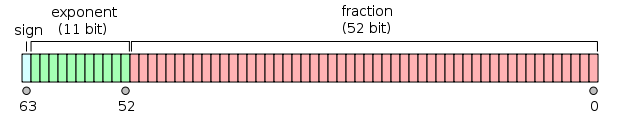
\includegraphics[width=0.85\textwidth]{618px_IEEE_754_Double_Floating_Point_Format}
    \caption[IEEE 754 Double Floating Point Format]{IEEE 754 Double Floating Point Format (Codekaizen / CC BY-SA 3.0 \cite{website:double_floating_point_image})}
    \label{double_floating_point_format}
\end{figure}

The representation of a number in the floating point format is therefore a chain of 64 binary digits (ones and zeros) that are interpreted as a real value as given by equation \ref{eq:64_bit_double_interpretation}.
\begin{equation} \label{eq:64_bit_double_interpretation}
(-1)^{sign}(1.b_{51}b_{50}...b_{0})_{2} \times 2^{e-1023} 
\end{equation}

Note that we can write the 64 binary digits more comfortably as 16 hexadecimal digits, where the first 3 encode the sign and the exponent and the remaining 13 the fraction. 

However there are some special definitions:

\begin{enumerate}
\item $0000 0000 0000 0000_{16}$ is defined as minus zero and $8000 0000 0000 0000_{16}$ as plus zero.
\item if the exponent is zero and the fraction is not zero the number is a subnormal and interpreted as:
\begin{equation}
(-1)^{sign}(0.b_{51}b_{50}...b_{0})_{2} \times 2^{1-1023} 
\end{equation}
\item $7FF0 0000 0000 0000_{16}$ is defined as Infinity and $FFF0 0000 0000 0000_{16}$ as minus Infinity
\item if the exponent has all ones in the binary representation and the fraction is not zero the encoded value is $NaN$.
\end{enumerate}

The smallest representable numbers in normalized form are those that have a one in the exponent and all zero in the fraction which evaluates to:

\begin{equation}
	\pm 2^{-1022} \approx \pm 2.22507 \times 10^{-308}
\end{equation}

The biggest possible finite numbers are those with the value 2046 in the exponent and all ones in the fraction which gives:

\begin{equation}
	\pm (1-2^{-53}) \times 2^{1024} \approx \pm 1.79769 \times 10^{308}
\end{equation}

The gap between two representable numbers depends on the exponent. Here are some examples:
\begin{itemize}
 \item	For the exponent 1023 we get the actual exponent 0. The possible range of representable numbers is from 1 to approximately 2. The gap between to neighbouring numbers is approximately $2.22045e-16$.
 \item For the exponent 1076 we get the actual exponent 53. The range is from 9007199254740992 to 18014398509481982 with a gap of 2 between representable numbers.
\end{itemize}

For the above two paragraph see also \cite{wiki:double_precision_floating_point} and \cite{wiki:ieee_745_1985}.

When working with floating point numbers you should be aware that most values can not be represented exactly, which can sometimes give unexpected results. Try to evaluate $0.3 - 0.2 - 0.1$ in the macro editor. The result is $-2.7756 * 10^ {-17}$. We did not introduce comparison operations yet. However considering the above it should be clear that you should not use equality or inequality operators with floating point numbers. Instead you should test if the difference between two values is reasonably small. The expression $ (0.3 - 0.2 - 0.1 == 0)$ would evaluate to {\tt false}. However considering that we gave the input numbers with one digit after the decimal point, indicating a precision of one tenth, the value $-2.7756 * 10^ {-17}$ is as close to zero as one could reasonably wish for. We should have therefore used an expression in the form of $ (0.3 - 0.2 - 0.1 < 0.01)$. 

\subsubsection{Calculations and Precedence}

The operators in table \ref{tbl:number_operations} have different precedence values. Operations with smaller precedence value are applied before operations with bigger precedence value, when an expression is evaluated. The operator precedence values reflect the usual multiplication before addition convention. You can change the order in which expressions are evaluated by using brackets. Subexpressions in brackets are evaluated first. Expressions in brackets can include brackets in which case the expressions in the innermost brackets are evaluated first. Listing \ref{lst:operator_precedence} shows some examples.

\begin{listing}[H]
\begin{minted}[frame=lines, linenos]{java}
(-1 + 3);
(-(1 + 3));
2 + 3 * 5;
(2 + 3) * 5;
\end{minted}
\caption{Examples for operator precedences.}
\label{lst:operator_precedence}
\end{listing}

\begin{enumerate}
\item[1-2] 	In line 1 the negation is executed first and the result is 2. In line 2 the addition is executed first and then the negation, leading to the result $-4$.
\item[3-4] Because of the operator precedence the multiplication is executed first in line 3. The result is 17. In line 4 the addition is executed first and the result is 25.
\end{enumerate}

\subsection{Strings}

Strings represent text. Besides of the comparison operations there is only one operator defined on strings. The operator has the symbol $+$ which stands in this case for the concatenation of strings. The concatenation means that the second string is appended to the first one so that the result is one string that begins with the first string, followed by the second string. As long as we only have string literals this is not very interesting. However as soon as we will use variables the situation will be different. The concatenation of strings is one of the most important operation in the ImageJ Macro Language. It will for example be needed to construct file names and paths and to construct parameters that are passed to commands or build in functions. Although there is only one operator on strings, there are a number of build in functions that we will discuss later. These allow for example to find and to replace substrings in strings.

To make it easier to represent the quote characters '' and ', a string literal can be embedded in either the double quotes or the single quotes. Some characters preceded by a backslash ({\tt \textbackslash}) have a special meaning and are called escape sequences. We already saw the newline ({\tt \textbackslash n}) and the tabulator ({\tt \textbackslash t}). The tabulator is not interpreted by the log-window but it can be useful when working with tables. Other useful escape sequences are ({\tt \textbackslash '}), ({\tt \textbackslash"}) and ({\textbackslash\textbackslash}). Besides of these the numerical ASCII code \cite{_ascii_code_1963} in octal form can be used, {\tt \textbackslash 040} is for example the octal code for the space character (32 in decimal notation).  

\begin{listing}[H]
\begin{minted}[frame=lines, linenos]{python}
"Hello" + " " + "World" + "!";
"Hello \"World\"!";
'Hello "World"!';
'\\n inserts a newline';
"\110\145\154\154\157\041";
\end{minted}
\caption{Examples for string literals, the concatenation operator and escape sequences.}
\label{lst:string_concatenation}
\end{listing}

\begin{listing}[H]
\begin{minted}[frame=lines, linenos]{text}
Hello World!
Hello "World"!
Hello "World"!
\n inserts a newline
Hello!
\end{minted}
\caption{The output produced by listing \ref{lst:string_concatenation}.}
\label{lst:string_concatenation_results}
\end{listing}

\subsection{Booleans}

Operators that operate on boolean values are the complement ({\tt !}), the conjunction operator or logical and ({\tt \&\&}) and the disjunction operator or logical or ({\tt ||}). The complement has the precedence one just like the numerical negation and the two other boolean operators have the precedence 5 so that when combining comparison operators with boolean operators and numerical operators the numerical operators are executed first, than the comparisons and at the end the boolean operators. 

The negation of {\tt false} is true and the negation of {\tt true} is  {\tt false}. The the result of the boolean and is one when both arguments are one and zero in all other cases and the boolean or is zero when both arguments are zero and one in all other cases. One use of the boolean operations is to combine different comparisons in a condition. Conditions will be needed for the conditional execution of code in if-statements and loops.

\begin{listing}[H]
\begin{minted}[frame=lines, linenos]{java}
"not";
(!false); 		1
(!true);		  0
"and";
(false && false);	 0
(false && true);	  0
(true && false);  	0
(true && true);   	1
"or"
(false || false);	 0
(false || true);	  1
(true || false);	  1
(true || true);	   1
\end{minted}
\caption{The boolean operations not, and and or.}
\label{lst:boolean_operations}
\end{listing}

Each table that maps the different combinations of input values {\tt false} and {\tt true} or 0 and 1 of the operands to a result value 0 or 1 defines a boolean operator. If we keep the order of the values for the operands fix, we can define an operation simply by giving the four different result values. And would for example be given by 0001 and or by 0111. There are 16 different possibilities for the four results with the two values 0 and 1. Each defines a different binary boolean operator. Some are rather trivial like 0000 and 1111. An exclusive or ({\tt xor}) that is true when exactly one of its operands is true would be given by 0110. Note that all the 16 different binary boolean operations can be expressed by only using {\tt and}, {\tt or} and {\tt not}. {\tt and}, {\tt or} and {\tt not} form a functionally complete set of boolean operators. In fact {\tt not} and {\tt and} or {\tt not} and {\tt or} alone do already form a complete set. And even the single operations {\tt nand} given by 1110 and {\tt nor} given by 1000 form each a complete set on its own.

If a and b are the parameters than the {\tt xor} operation can be expressed by the expression \texttt{((!a \&\& b) || (a \&\& !b))}. You can prove this by putting in the different combinations of possible values and comparing the resulting truth table with that of the {\tt xor} operation.

\begin{listing}[H]
\begin{minted}[frame=lines, linenos]{java}
((!(false) && false) || (false && !(false)));	0	
((!(false) && true) || (false && !(true)));	  1
((!(true) && false) || (true && !(false)));	  1
((!(true) && true) || (true && !(true)));	    0
\end{minted}
\caption{The boolean operations xor expressed with and, or and not.}
\label{lst:boolean_operation_xor}
\end{listing}

Given the truth table of an operation you can find the equivalent expression with {\tt and}, {\tt or} and {\tt not} systematically in the following way. For each row in the result column that contains a one build an expression by negating the operands if they are zero and by not negating them if they are one. Combine the operands using {\tt and} and the sub--expressions for the rows by using {\tt or}. For example the truth table for {\tt xor} is one for 01 which gives the sub--expression \texttt{(!a \&\& b)}. The only other one is for the row 10 with gives the sub--expression \texttt{(a \&\& !b)}. Now the two sub-expressions need to be combined by or which gives  \texttt{((!a \&\& b) || (a \&\& !b))}.

Another useful property is the duality of {\tt and} and {\tt or}. This means if you have an expression containing only {\tt and} and {\tt not} you can obtain an equivalent expression containing only {\tt or} and {\tt not} by replacing every {\tt and} with and {\tt or} if you negate each operand and the result of the operation.

\begin{equation}
	\tt{a \&\& b} = \tt{!(!a || !b)}
\end{equation}

and

\begin{equation}
	\tt{a || b} = \tt{!(!a \&\& !b)}
\end{equation}
 
\begin{listing}[H]
\begin{minted}[frame=lines, linenos]{java}
(!(!false || !false));	 0
(!(!false || !true)); 	 0
(!(!true || !false)); 	 0
(!(!true || !true));  	 1

(!(!false && !false));	 0
(!(!false && !true)); 	 1
(!(!true && !false)); 	 1
(!(!true && !true));  	 1
\end{minted}
\caption{The duality of {\tt and} and {\tt or}.}
\label{lst:boolean_operation_duality}
\end{listing}

\subsection{Numbers as Bit-Strings}

There is a number of operations that work on the internal binary representation of the integer part of numbers. 

\begin{center}
\begin{tabular}{|l|l|l|l|p{3cm}|}
\hline
Operator & Precedence & Result Type & Name & Description \\ \hline
\textasciitilde & 1 & number & bitwise complement & unary operator that changes each 0 to 1 and each 1 to 0 \\ \hline
\textbar & 2 & number & bitwise or & only zero if both bits are zero \\ \hline
\textasciicircum & 2 & number & bitwise exclusive or & one is exactly one bit is one  \\ \hline
\& & 2 & number & bitwise and & one if both bits are one \\ \hline
\textless\textless & 2 & number & left shift & shifts the bits of the first operand a number of places give by the second operand to the left \\ \hline
\textgreater\textgreater & 2 & number & right shift & shifts the bits of the first operand a number of places give by the second operand to the right \\ \hline
\end{tabular}
\captionof{table}{Operators that operate on the binary representation of the integer part of numbers.}
\label{tbl:number_binary_operations}
\end{center}

These operations work on the binary representation of integer numbers in java. Note that in the ImageJ Macro Language all numbers are represented as floating point numbers. However when you use the above operations the integer part of the number is converted internally to integer. To fully understand how they work we need to know how integer values are represented in java. 

\subsubsection{Two's complement representation of integer values}

Integer values use 32 bits or four bytes in java and can therefore encode $2^{32} = 4294967296$ different values. Since the 32 bits are long to write each of the 4 bytes is often written as a two digit hexadecimal number. However to demonstrate the principle we will use just 3 bits. We could of course just use all three bits to binary encode the numbers from 0 to 7. But then we could not represent negative numbers. So we could reserve the leftmost bit to represent the sign with 0 indicating a positive number and 1 a negative number. This is called the signed magnitude representation. It has two disadvantages. First there are two representations for 0 and second the binary arithmetic is not straightforward since case distinctions depending on the sign must be made. A better representation is the one's complement. The positive numbers are represented as before. A negative number is build from its positive counterpart by applying the bitwise complement operation. This results in the encodings in table \ref{tbl:signed_magnitude}. Calculations using the one's complement are simpler. The binary numbers can for example be added in the usual way, only when a carry at the leftmost position occurs it has to be added back at the rightmost position. However there are still to representations for zero. 

\begin{center}
\begin{tabular}{rcc}
decimal & binary signed magnitude & binary one's complement  \\
-3 & 111 & 100 \\
-2 & 110 & 101 \\
-1 & 101 & 110 \\
-0 & 100 & 111 \\
+0 & 000 & 000 \\
+1 & 001 & 001 \\
+2 & 010 & 010 \\
+3 & 011 & 011 \\
\end{tabular}
\captionof{table}{Signed magnitude representation and one's complement with 3 bits.}
\label{tbl:signed_magnitude}
\end{center}
      
We can get simpler binary arithmetic and unique representations by using the two's complement. The positive numbers are still encoded as before. The negative counterpart of a positive number is created by building the one's complement and adding one to the result. 

\begin{center}
\begin{tabular}{rcc}
decimal & binary one's complement & binary two's complement  \\
-4 &     & 100 \\
-3 & 100 & 101 \\
-2 & 101 & 110 \\
-1 & 110 & 111 \\
-0 & 111 &     \\
+0 & 000 & 000 \\
+1 & 001 & 001 \\
+2 & 010 & 010 \\
+3 & 011 & 011 \\
\end{tabular}
\captionof{table}{One's complement and two's complement with 3 bits.}
\label{tbl:twos_complement}
\end{center}

\subsubsection{Bitwise operations}

The \textit{bitwise complement} operation changes each bit in the two's complement representation of the number from 0 to 1 or from 1 to 0. For example the bitwise complement of 3 is --4. The binary representation of 3 is 011. Inverting each bit yields 100 which encodes -4 in two's complement representation. Of course our real integer representation uses 32 bits. Note that the bitwise complement of a number x is $-x-1$ if the numbers are represented in two's complement as is the case here. The \textit{bitwise or} will calculate the logical or for each position in the representation of the two numbers. For example: $(-3 | 3)$ gives $-1$. The binary representations of --3 and 3 are $101$ and $011$. The bitwise or results in $111$ which is the two's complement representation of -1. For the \textit{exclusive or} the result is one if exactly one of the bits is one. $(-3 ^ 3)$ gives $-2$, since the resulting representation is $110$. The representation of the result of the \textit{bitwise and} will have a one at each position at which the representations of both operands have a one. For example: $3 \& -2$ gives $2$. The binary representation of 3 is $011$. The representation of --2 is $110$. The result of the bitwise and is $010$ which encodes 2. The \textit{shift operations} move the bits n positions to the left or to the right. When shifting to the right the highest bit is preserved, when shifting to the left zeros are filled in for the missing values. In the binary representation each digit signifies a power of two. Shifting by n positions is therefore equivalent to multiplying or dividing (integer division) by $2^{n}$. $256>>2$ results in 64 and $7<<3$ gives 56.

Sometimes the different bytes of a number are used to encode independent values. This is for example the case for the {\tt setPixel(x,y,v)} and {\tt getPixel(x,y)} build-in functions of ImageJ that in case of RGB images use one single number for an RGB-color value. The bitwise-operations can then be used to retrieve and set the independent parts easily.
The rightmost byte (eight bits) encodes the blue value, the next one to the left the green value and the one before this one the red value. The leftmost byte is unused. 

\begin{listing}[H]
\begin{minted}[frame=lines, linenos]{java}
0xFFA900;	// color value that encodes a shade of orange

(0xFFA900>>16) & 0xFF; // red
(0xFFA900>>8)  & 0xFF; // green
0xFFA900       & 0xFF; // blue

0 | (169<<8)  | (255<<16); // create composite value from components

setForegroundColor(0xFFA900);
\end{minted}
\caption{Encoding and decoding of rgb-components in one integer value with the help of bit-operations.}
\label{lst:bit_operations_example}
\end{listing}

\subsection{Comparison Operations}

The comparison operations are defined for all basic datatypes: numbers, booleans and strings. The available operations are \textit{less than} ({\tt \textless}), \textit{less than or equal} ({\tt \textless =}), \textit{greater than} ({\tt \textgreater}), \textit{greater than or equal} ({\tt \textgreater =}), \textit{equal} ({\tt ==}), \textit{not equal} ({\tt !=}). Note that the comparison operations have the precedence 4, so that they are evaluated after calculations and before the boolean operations.

\begin{listing}[H]
\begin{minted}[frame=lines, linenos]{java}
(false < true);		 1
(true <= true);		 1
(7>5);			  1
(0.123 < 0.12300000001);	1
(NaN != NaN);		   1
("a"<"b");		      1
("fox"<"horse");		1
("yes"=="yes")		  1
(parseFloat("Infinity")>9999999999);		 1
(parseFloat("-Infinity")<9999999999);		1
(parseFloat("Infinity")>(parseFloat("-Infinity")));  1
(parseFloat("Infinity")==parseFloat("Infinity"));    1
\end{minted}
\caption{Examples of comparisons.}
\label{lst:comparisons}
\end{listing}

Note line 5 in listing \ref{lst:comparisons}. $NaN$ is not equal to $NaN$. The IEEE 754\cite{_754-2008_2008} specifies: 
\begin{quotation}
 ''All numeric operations with NaN as an operand produce NaN as a result. As has already been described, NaN is unordered, so a numeric comparison operation involving one or two NaNs returns false and any != comparison involving NaN returns true, including x!=x when x is NaN''.
\end{quotation}

If you want to test if a value is $NaN$, you should use the build--in function {\tt isNaN()}.

\section{Variables and Assignments}

Only working with literal values will not take us very far. We need to write down the same expression each time we want to evaluate it for different values. The solution to this are variables. Variables are an important concept in programming. A variable has an identifier (the name of the variable) and a value that has been assigned to the variable with the help of an assignment operator. Variables can be used in expressions in the way as literals. Variables allow us to generalize and to write expressions independent from the concrete values for which they will be evaluated.

The identifier of a variable must only contain letters, digits and the underscore (''\_'') character. It must not begin with a digit. Identifiers are case-sensitive, meaning that for example the lower-case letter ''x'' will be considered a different variable from the upper-case letter ''X''.

Before a variable can be used in an expression it must be defined by assigning it a value. This is done with the help of the assignment operator ({\tt =}). At the left side of the assignment must be a variable and at the right side an expression. The expression can contain variables itself and even the same variable as on the left side if it had already been defined before. When the assignment expression is evaluated, the variables on the right side are replaced by their values before the expression on the right side is evaluated. The result is then assigned to the variable on the left side.

\begin{listing}[H]
\begin{minted}[frame=lines, linenos]{java}
radius = 11.25;
circumference = 2 * PI * radius;
area = PI * radius * radius;
print("radius:", radius, "circumference:", circumference, "area:", area);
\end{minted}
\caption{Calculation of the area and circumference of a circle with the help of variables. Note that PI is not a variable, but a build in constant.}
\label{lst:circle_with_variables}
\end{listing}

\begin{listing}[H]
\begin{minted}[frame=lines, linenos]{text}
radius: 7.25 circumference: 45.5531 area: 165.13
radius: 9.25 circumference: 58.1195 area: 268.8025
radius: 11.25 circumference: 70.6858 area: 397.6078
\end{minted}
\caption{Output of listing \ref{lst:circle_with_variables} after changing the radius and running the script multiple times.}
\label{lst:circle_with_variables_output}
\end{listing}

It is important to remember that assignment statements with a variable on the right side, assign the value of the right-hand variable to the variable on the left side as long as basic datatypes are used. They do not create a reference to the right hand variable. This will be different for arrays as we will see later. 

\begin{listing}[H]
\begin{minted}[frame=lines, linenos]{java}
balanceA = 1000;
balanceB = balanceA;
balanceB = balanceB + 500;
print("balance A: ", balanceA, "balance B: ", balanceB);
\end{minted}
\caption{The output of the macro is ''balance A: 1000 balance B: 1500''. Note that {\tt balanceA} has not been changed when {\tt balanceB} has been modified.}
\label{lst:copy_by_value}
\end{listing}

There is a number of operators that works on variables. We already saw the assignment operator that assigns a value to a variable. As a shortcut for expressions that contain the same variable on the right and on the left side of the assignment there are the operators $+=$, $-=$, $*=$ and $/=$. $a += 2$ is for example a shortcut for $a = a + 2$, etc.

Furthermore there are the pre and post increment and decrement operators that increment and decrement the value of a variable either before the evaluation of the expression or afterwards.

\begin{listing}[H]
\begin{minted}[frame=lines, linenos]{java}
a = 5;
b = a++ + 3;
c = 5;
d = ++c + 3
print("b:", b, "a:", a);	b: 8 a: 6
print("d:", d, "c:", c);	d: 9 c: 6
\end{minted}
\caption{The post- and pre- increment operations.}
\label{lst:post_increment}
\end{listing}

\begin{center}
\begin{tabular}{|l|l|l|l|p{3cm}|}
\hline
Operator & Precedence & Result Type & Name & Description \\ \hline
++ & 1 & number & pre- or postincrement & unary operator that adds one to the value of the variable either before the evaluation of the containing expression (preincrement) or afterwards (postincrement) \\ \hline
$--$ & 1 & number & pre- or postdecrement & unary operator that subtracts one from the value of the variable either before the evaluation of the containing expression (predecrement) or afterwards (postdecrement) \\ \hline
+= & 6 & number & assignment with addition & add the value on the right hand of the expression to the variable  \\ \hline
-= & 6 & number & assignment with subtraction & subtract the value on the right hand of the expression from the variable  \\ \hline
*= & 6 & number & assignment with multiplication & multiply the variable with the value on the right hand of the expression\\ \hline
/= & 6 & number & assignment with division & divide the variable by the value on the right hand of the expression \\ \hline
\end{tabular}
\captionof{table}{Operators on variables.}
\label{tbl:variable_operations}
\end{center}

\subsection{Automatic type conversion}

When using the {\tt +} operator a number can sometimes be automatically converted into a string. This allows to easily construct messages which contain the numerical values of variables. It works when the first operand is a string. If the first operand is a number the second operand is expected to be a number as well and an error will occur.

\begin{listing}[H]
\begin{minted}[frame=lines, linenos]{java}
r = 6.4;
message = "radius: " + r + "cm";
print(message);
message = toString(r) + "cm is the radius";
print(message);
message = "" + r + "cm is the radius";
print(message);
\end{minted}
\caption{A number is automatically converted into a string when the first operand of the + operator is a string.}
\label{lst:auto_conversion}
\end{listing}

\subsection{Arrays}

Arrays are lists of values. In the ImageJ Macro Language the different elements in an array can be of different types. When an array is created it is usually assigned to a variable. An element of the array is read or changed by using an index. The first index is zero and the last index of an array with the length $l$ is $l-1$. 

\begin{listing}[H]
\begin{minted}[frame=lines, linenos]{java}
primeNumbers = newArray(3, 5, 7, 11, 13, 17, 19, 23);
print(primeNumbers[0]);					3
print(primeNumbers[primeNumbers.length-1]);		   23

options = newArray(34, true, "Huang");
print("threshold value:", options[0]);
print("dark background:", options[1]);
print("threshold method:", options[2]);
\end{minted}
\caption{Two examples of arrays.}
\label{lst:arrays}
\end{listing}

Note that arrays are assigned to variables by reference not by value. This means when you have assigned an array to multiple variables, the same array is modified via each variable. 

\begin{listing}[H]
\begin{minted}[frame=lines, linenos]{java}
labels = newArray("one", "TOO", "three", "four");
correctLabels = labels;
correctLabels[1] = "two";
print(correctLabels[1]);	two
print(labels[1]);	       two
\end{minted}
\caption{Arrays are assigned by reference.}
\label{lst:arrays_assigned_by_reference}
\end{listing}

Arrays can either be created by listing the containing values or by giving the size of the array. In the second case all elements of the array are initialized with the value 0.

\begin{listing}[H]
\begin{minted}[frame=lines, linenos]{java}
a = newArray(3);
print(a[0]);		0
a[0] = "one";
a[1] = "two";
a[2] = "three";
print(a[1]);		two
\end{minted}
\caption{Creation of an ''empty'' array with a given size.}
\label{lst:empty_array}
\end{listing}

\section{Conditional code execution}

A program must be able to react differently depending on the input values or its current internal state. This can be achieved by the if/then/else statement. In the ImageJ Macro Language it has the form shown in Listing \ref{lst:if_then_else}.

\begin{listing}[H]
\begin{minted}[frame=lines]{java}
if (condition) {
	list of statements 1
} else {
	list of statements 2
}
\end{minted}
\caption{The form of the if/then/else statement}
\label{lst:if_then_else}
\end{listing}

The condition must evaluate to a boolean value. If the condition is true, the statements in the first block enclosed in curly brackets is executed, otherwise the statements in the else--block are executed. The else-part of the statement is optional and can be omitted. 

The then--block and the else--block can contain other if statements, however you should avoid this as far as possible since programs with nested if-statements are difficult to understand. Note furthermore that when variables are defined in a then--block or else--block, they will only be defined in the following program, if the execution passed by the corresponding block. You should only define variables within a then- or else-block if it is exclusively used within that block, otherwise you should define the variable outside the if-statement (you can than use it within).

\begin{listing}[H]
\begin{minted}[frame=lines, linenos]{java}
a = getNumber("Enter a number: ", 13);
if (a%2==0) {
	print(a + " is even");
}
else { 
	print(a + " is odd");
}
\end{minted}
\caption{Simple example of the if/then/else statement.}
\label{lst:example_if}
\end{listing}

Listing \ref{lst:example_if} shows a simple example. The build-in function {\tt getNumber} is used to get a number $a$ from the user. The condition of the if-statement tests if $a$ is even by using the modulo operator. $a$ is even if $a$ modulo 2 is zero. In this case the first block is executed. In this example the list of statements in the block consists of only one statement, which prints out the message ''$a$ is even''. If the condition evaluates to false, i.e. if $a$ modulo 2 is different from zero, the else-block is executed. It prints out the message ''$a$ is odd''. Note that when a block contains only a single statement the curly brackets can be omitted. However this is not advisable since it can lead to errors when modifying the code later.

Listing \ref{lst:example_if_abs} shows an other example. This time the curly brackets have been omitted.

\begin{listing}[H]
\begin{minted}[frame=lines, linenos]{java}
a = getNumber("Enter a number", -3);
if (a<0) 
	result = -a;
else 
	result = a;
print( "abs(" + a + ")=" + result); 
\end{minted}
\caption{Another example of a simple if-statement.}
\label{lst:example_if_abs}
\end{listing}

This example calculates and displays the absolute value of the entered number. If $a$ is smaller than zero the result is the negation of $a$ and therefore positive, otherwise the result is $a$.

We can use the if-statement to calculate the maximum of two numbers $a$ and $b$. If $a$ is larger than or equal to $b$ the result is b and otherwise the result is $b$. The corresponding code is shown in Listing \ref{lst:example_if_max}.

\begin{listing}[H]
\begin{minted}[frame=lines, linenos]{java}
a = 10;
b = 4;
if (a>=b) 
	result = a;
else 
	result = b;
print("max("+a+", "+b+")=" + result);
\end{minted}
\caption{Calculation of the maximum of two numbers.}
\label{lst:example_if_max}
\end{listing}

Listing \ref{lst:example_if_key} shows a more complex example of an if-statement. This time the code contains multiple if-statements. The else-parts have been omitted. The then-blocks contain more than one statement and one of the if-statements is nested, i.e. its then-block contains another if-statement.

\begin{listing}[H]
\begin{minted}[frame=lines, linenos]{java}
waitForUser;
shiftPressed = isKeyDown("shift");
altPressed = isKeyDown("alt");
message = "keys pressed: ";
counter = 0;
if (shiftPressed) {
	message = message + "SHIFT";
	counter++; 
}
if (altPressed) {	
	if (counter>0) message = message + ", ";
	message = message + "ALT";
	counter++; 
}
if (counter==0) message = message + " NONE";      
print(message);
\end{minted}
\caption{Using the if-statement to test which modifier keys are pressed.}
\label{lst:example_if_key}
\end{listing}

The macro will display which of the modifier keys {\tt SHIFT} and {\tt ALT} are pressed. The {\tt waitForUser}-command pauses the execution of the macro until the user clicks the {\tt ok}-button on the dialog that the command opens. This gives you the possibility to press and hold down the modifier keys. The {\tt isKeyDown} build-in function will answer {\tt true} if the specified key is pressed. At the end a message indicating that either none of the keys, the shift-key, the alt-key or both have been pressed. The nested if, in the if-statement that tests if the alt-key is pressed, allows to add a comma in the case that both keys are pressed. Note that it would be bad style to write the condition as ''{\tt if (shiftPressed==true) ...}''. The variable is already boolean and it is unnecessary to compare it to {\tt true} or {\tt false}.

In Listing \ref{lst:example_if_var} the variable $b$ is defined in the then-block of the if-statement. Running the macro will produce an error. Since $a$ is zero the execution does not pass into the then-block of the first if-statement and $b$ will be undefined in the condition of the second if-statement. To correct the macro $b$ should be defined at the top of the macro for example with the expression $b = 0;$. 

\begin{listing}[H]
\begin{minted}[frame=lines, linenos]{java}
a = 0;
if (a>0) {
	b=2;
}
if (b>1) {
	c=3;
}
print(c);
\end{minted}
\caption{The example will produce an error because b will be undefined in line 5.}
\label{lst:example_if_var}
\end{listing}

\section{Loops}

A loop allows to repeatedly execute a code block. A condition is evaluated for each iteration of the loop and decides when the loop finishes. In image processing loops can for example be used to load each image from a given folder or to apply an operation to each pixel of an image. In the ImageJ Macro Language there are three different forms of loops. the for-loop, the while-loop and the do-while-loop.

\subsection{The for--loop}

The for-loop is preferably used when the number of iterations is known from the start. It has the form shown in Listing \ref{lst:form_for_loop}.

\begin{listing}[H]
\begin{minted}[frame=lines, linenos]{java}
for (initialization; condition; increment) {
	list of statements
}
\end{minted}
\caption{The form of a for-loop.}
\label{lst:form_for_loop}
\end{listing}

The  {\tt initialization} is executed one time at the beginning, before the loop is entered. It is normally used to initialize the counter variable of the loop. The {\tt condition} is evaluated before each iteration of the loop. If it evaluates to {\tt true} the loop is entered, otherwise the execution of the code continues after the body of the loop. The {\tt condition} usually tests if the counter variable of the loop has reached a specific value. The {\tt increment} is executed after each iteration of the loop. It is usually used to modify the counter variable of the loop.

Listing \ref{lst:simple_for_loop} shows a basic example of a for-loop. The macro prints the numbers from one to ten.

\begin{listing}[H]
\begin{minted}[frame=lines, linenos]{java}
for (i=1; i<11; i++) {
	print(i);
}
\end{minted}
\caption{The loop prints the numbers from one to ten.}
\label{lst:simple_for_loop}
\end{listing}

Listing \ref{lst:for_loop_even} prints out the even numbers from two to ten. It increments the counter variable of the loop by two in the {\tt increment}. Let us see how this is executed. The first time the execution reaches the loop, $i$ is initialized to $2$. The {\tt condition} is executed and since $2<11$ evaluates to {\tt true}, the body of the loop is entered. The value of $i$ which is currently $2$ is printed. The {\tt increment} is executed and adds $2$ to the current value of $i$ so that $i$ has now the value $4$. Now the {\tt condition} is executed with $i=4$ and evaluates to {\tt true}. The execution enters the body of the loop, and so on. After $6$ iterations $i$ reaches the value $12$. This time the condition evaluates to {\tt false} and the execution continues after the body of the loop.

\begin{listing}[H]
\begin{minted}[frame=lines, linenos]{java}
for (i=2; i<11; i+=2) {
	print(i);
}
\end{minted}
\caption{The loop prints the even numbers from two to ten.}
\label{lst:for_loop_even}
\end{listing}

In the next example the counter variable of the loop starts with a high number and counts down to 2. This macro calculates the nth factorial, i.e. the multiplication of the numbers from one to $n$. Remember that $i--$ means $i = i - 1$ and $factorial *= i$ stands for $factorial = factorial * i$. In the first iteration $factorial$ is one and $i$ five. $factorial$ becomes five. In the next iteration $factorial$ is five and $i$ four. And so on. In the last iteration $i$ is two while $factorial$ is $5 * 4 * 3 = 60$. 

\begin{listing}[H]
\begin{minted}[frame=lines, linenos]{java}
n = 5;
factorial = 1;
for (i=n; i>1; i--) {
	factorial *= i;
}
print(factorial);
\end{minted}
\caption{Calculation of the nth factorial.}
\label{lst:for_loop_factorial}
\end{listing}

Loops are often used to process each element of a given list of elements. This can for example be the numbers in an array or the files and sub--folders in a folder. When iterating over the elements of an array, you must remember that the index of the first element is zero. If the array contains $l$ elements, the index of the last element is $l-1$. If {\tt numbers} is a variable containing an array, {numbers.length} returns the number of elements in the array {\tt numbers}.

The example in Listing \ref{lst:for_loop_square} replaces each element of the array by the square of the element. The build-in function Array.print is used to print all elements of the array at the end. 

\begin{listing}[H]
\begin{minted}[frame=lines, linenos]{java}
numbers = newArray(1,2,3,4,5,6,7,8,9,10);
for(i=0; i<numbers.length; i++) {
	numbers[i] = numbers[i] * numbers[i];
}
Array.print(numbers);
\end{minted}
\caption{Squaring each element in an array.}
\label{lst:for_loop_square}
\end{listing}

The next example will print the names of files and sub-folders in your home folder, each in a separate line. The macro uses the build-in function {\tt getDirectory} with the parameter {\tt "home"}. This answers the path to the user's home folder. The path is then passed to the function {\tt getFileList}, which will return an array of the names of files and folders in the given folder. The loop iterates over this array and prints each element.

\begin{listing}[H]
\begin{minted}[frame=lines, linenos]{java}
home = getDirectory("home");
files = getFileList(home);
for (i=0; i<files.length; i++) {
	file = files[i];
	print(file);
}
\end{minted}
\caption{Printing the files and folders in the user's home folder.}
\label{lst:for_loop_home}
\end{listing}

Note that each part {\tt initialization}, {\tt condition} and {\tt increment} can be missing. If the condition is missing the only way to exit the loop is to exit the whole macro with an error by using the {\tt exit} command. 

\begin{listing}[H]
\begin{minted}[frame=lines, linenos]{java}
i=2;
for (; ; ) {
	print(i);
	if (i>=10) exit("FINISHED");
	i+=2;
}
print("EXECUTION WILL NEVER PASS HERE");
\end{minted}
\caption{A loop with empty an empty {\tt initialization}, {\tt condition} and {\tt increment}.}
\label{lst:for_loop_empty}
\end{listing}

The for-loop in Listing \ref{lst:for_loop_empty} prints out the even numbers from two to ten. When ten is reached the macro is stopped with an error. Since the {\tt condition} of the loop is empty, this is the only way to exit the loop. 

The {\tt initialization} and the {\tt increment} can use other variables as the counter of the loop and the {\tt condition} can be any expression that evaluates to a boolean value. However you should normally avoid to such use such unusual style, because it can easily misinterpreted by others or yourself when you come back to the code later.

Listing \ref{lst:for_loop_game} implements a simple number guessing game. The game is over either when the player guessed the right number or when he made ten wrong guesses. A for-loop is used since the maximal number of trials is known beforehand, however the condition checks not only the counter variable but also a flag that indicates if the player has won the game.

\begin{listing}[H]
\begin{minted}[frame=lines, linenos]{java}
number = floor(100 * random) + 1;
guess = getNumber("Guess my number between 1 and 100: ", 50);
won = false;
for(i=1; ((i<10) && !won); i++) {
  if (guess==number) {
    showMessage("you won!");
    won = true;
  } else {
    if (number<guess) message = "my number is smaller, try again: ";
    else message = "my number is bigger, try again: "; 
    guess = getNumber(message, guess);
  }
}
if (!won) showMessage("I won!"); 
\end{minted}
\caption{A simple number guessing game.}
\label{lst:for_loop_game}
\end{listing}

We will now iterate over all pixels of a two-dimensional image. To demonstrate this, we will create a new empty image and then create a pattern on it, by setting each pixel to a value, depending on its coordinates in the image. Since we can easily access the width and the height of the image and since we can specify the pixel coordinates by their $x$ and $y$ positions, the easiest way is to use a nested for-loop. The outer loop iterates over one dimension and the inner-loop over the other. Note that if the outer loop runs from $0$ to $N-1$ and the inner loop from $0$ to $M-1$, the body of the inner loop is executed $N \times M$ times. It can therefore be important to not do unnecessary things in the body of the inner loop.

\begin{listing}[H]
\begin{minted}[frame=lines, linenos]{java}
newImage("pattern", "8-bit", 255, 255, 1);
width = getWidth();
height = getHeight();
for(x=0; x<width; x++) {
    for(y=0; y<height; y++) {
    	setPixel(x, y, x*y % 255);
    }
}
\end{minted}
\caption{Looping over the pixels of an image.}
\label{lst:for_loop_pixels}
\end{listing}

Listing \ref{lst:for_loop_pixels} will produce an image similar to that in Figure \ref{fig:pattern}.

\begin{figure}[h!]
  \centering
    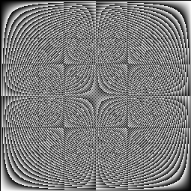
\includegraphics[width=0.4\textwidth]{pattern}
    \caption[A pattern created by the example macro]{The pattern created by the example macro in Listing \ref{lst:for_loop_pixels}.}
    \label{fig:pattern}
\end{figure}

Instead of creating a pattern, we can modify the pixel values of an existing image. Listing \ref{lst:for_loop_invert} shows an example that uses a nested for-loop to invert the contrast of an 8-bit image, by replacing each pixel value $v$ by $255-v$. You need to open an 8-bit image before running this macro. You can for example use the bridge-example-image from the menu {\tt File>Open Samples>Bridge (174K)}.

\begin{listing}[H]
\begin{minted}[frame=lines, linenos]{java}
width = getWidth();
height = getHeight();
for(x=0; x<width; x++) {
    for(y=0; y<height; y++) {
    	value = getPixel(x, y);
    	setPixel(x, y, 255-value);
    }
}
\end{minted}
\caption{Using a nested for-loop to invert the contrast of an 8-bit image.}
\label{lst:for_loop_invert}
\end{listing}

By changing the position of an object in an image in a loop we can create an animation. The example in Listing \ref{lst:for_loop_animation} creates a region of interest in the upper left corner of the image and moves it along the diagonal until it leaves the image in the lower right corner. Depending on the speed of your machine, you might need to change the argument of the {\tt wait} command. The {\tt wait} command will cause ImageJ to pause for the given time in milliseconds before the execution continues. Without it the macro might run to fast to see the animation. 

\begin{listing}[H]
\begin{minted}[frame=lines, linenos]{java}
newImage("animation", "8-bit", 800, 800, 1);
makeOval(0,0,20,20);
Roi.setFillColor("red");	
for(i=0; i<800; i++) {
	Roi.move(i, i);
	wait(20);
}
\end{minted}
\caption{Using a for-loop to create an animation.}
\label{lst:for_loop_animation}
\end{listing}

\subsection{The while--loop}

The while-loop has the form shown in Listing \ref{lst:while_loop}. Before the body of the loop is entered, the condition is executed. If it evaluates to true, execution continues in the body of the loop. When the execution reaches the end of the body of the loop, the condition is evaluated again. If it still evaluates to true the body of the loop is entered again, otherwise the execution continues after the body of the loop.

\begin{listing}[H]
\begin{minted}[frame=lines, linenos]{java}
while(condition) {
  list of statements
}
\end{minted}
\caption{The form of the while-loop.}
\label{lst:while_loop}
\end{listing}

It is clear that While- and for-loop are equivalent in the sense that for every while-loop there is a for-loop that can simulate it and vice versa. To simulate a while-loop by a for loop it is sufficient to use the condition of the while-loop in the for-loop and to leave the initialization and increment empty. A for-loop can be simulated by a while-loop by putting the initialization directly before the loop and the increment as the last statement in the body of the loop.

While-loops are preferably used when the number of times the loop will run is not known at the beginning. This is for example the case when calculating an iterative approximation of a function. We can for example calculate the square root of a given number using Newton's method. According to Newton's method if we have an initial approximation $A$ for the value of the square root of $N$ we get a better approximation by dividing $N$ by $A$, adding $A$ to the result and dividing the result by $2$. 

\begin{equation}
	A_{i+1} = {{1}\over{2}} \cdot {({{N} \over {A_{i}}} + A_{i})}  
\end{equation}

We do not now beforehand how many iterations we will need until the result is good enough. However since we can easily calculate the square we can test if $A^{2}$ is sufficiently close to $N$ and in this case we know that we can stop iterating. 

\begin{listing}[H]
\begin{minted}[frame=lines, linenos]{java}
input = 121;
guess = 1;
nr_iterations = 0;
while(abs((guess*guess) - input) > 0.000001) {
	guess = 0.5 * ((input / guess) + guess);
}
print(guess);
\end{minted}
\caption{Calculation of the square root using Newton's method.}
\label{lst:while_loop_square_root}
\end{listing}

Another example is to calculate the number of times a given number can be divided by 2 using integer division until the result is 1. For example:
\begin{align}
	9 = 2 \times 4  + 1  \\
	4 = 2 \times 2 + 0 \\
	2 = 2 \times 1 + 0
\end{align}
So the answer for the input nine is three. Note that this corresponds to the integer part of the logarithm to the basis 2. Here again we do not know beforehand how many iteration are needed.

\begin{listing}[H]
\begin{minted}[frame=lines, linenos]{java}
n = 128;
counter = 0;
while(n>1) {
	n = floor(n / 2);
	counter++;
}
print(counter);
\end{minted}
\caption{Calculation of the integer part of the logarithmus dualis.}
\label{lst:while_loop_log_dualis}
\end{listing}

As a last example we will present a random walk that stops when it reaches the border of the image. Imagine an object in the middle of the image. In each step the object moves a given distance in a random direction, either up, down, left or right and leaves a trace while moving. Since the direction is random in each step, we can not know after how many iterations the object will reach the border of the image.

\begin{listing}[H]
\begin{minted}[frame=lines, linenos]{java}
newImage("random-walk", "8-bit", 800, 800, 1);
x = 400;
y = 400;
makeOval(x,y,20,20);
moveTo(x,y);
Roi.setFillColor("green");	
while(x>=0 && x<800 && y>=0 && y<800) {
	x = x + 10 * round((2 * random) -1); 
	y = y + 10 * round((2 * random) -1); 
	Roi.move(x, y);
	lineTo(x,y);
	wait(10);
}
\end{minted}
\caption{A random walk that stops when the border of the image is reached.}
\label{lst:while_random_walk}
\end{listing}

Note that the way we implemented the random walk the object can actually stay at its current coordinates for some steps, since the increment for the coordinates can be zero. You can see an example of a random walk in Figure \ref{fig:random_walk}. 

\begin{figure}[h!]
  \centering
    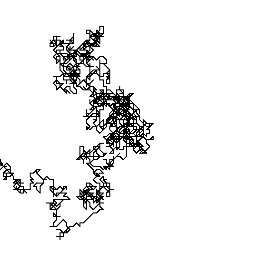
\includegraphics[width=0.4\textwidth]{random_walk}
    \caption[A random walk]{The image created by the random walk in Listing \ref{lst:while_random_walk}.}
    \label{fig:random_walk}
\end{figure}

\subsection{The do--while--loop}

The do--while--loop works similar as the while--loop. However in this case the condition is evaluated after each iteration and not before. This means that other as for the while--loop the body of the do--while--loop is guaranteed to be executed at least once. The form of the do--while--loop is shown in Listing \ref{lst:do_while_loop}. 

\begin{listing}[H]
\begin{minted}[frame=lines, linenos]{java}
do {	
	list of statements
} while (condition);
\end{minted}
\caption{The form of the do--while--loop.}
\label{lst:do_while_loop}
\end{listing}

Note that the do--while--loop can be simulated by a while--loop, by copying the content of the body of the loop one time before the beginning of the loop. In the example in Listing \ref{lst:do_while_example} the user is asked for a number between zero and one. The loop continues until the user enters a number fulfilling this condition.

\begin{listing}[H]
\begin{minted}[frame=lines, linenos]{java}
do {
   n = getNumber("Enter a number between 0 and 1", 0.5);
 } while (n<0 || n>1);
 print("number:", n);
 \end{minted}
\caption{Using the do--while--loop to obtain valid input.}
\label{lst:do_while_example}
\end{listing}

\section{User--defined functions}

In the ImageJ Macro Language you can define your own functions. A function is a block of code that has a name and a number of arguments. When the function is called, the arguments are replaced by the values in the call and the body of the function is executed. A function can have a return value. If this is the case the function call can be used on the right-side of an assignment statement or as the parameter of another function call. Listing \ref{lst:fct_definition} shows the form of a function definition.

\begin{listing}[H]
\begin{minted}[frame=lines, linenos]{java}
function name(list of arguments) {
	list of statements
}
\end{minted}
\caption{The form of a function definition.}
\label{lst:fct_definition}
\end{listing}

In Listing \ref{lst:for_loop_factorial} we used a for--loop to calculate the factorial of a number $n$. Remember that the factorial of the number $n$ is the product of the numbers from $1$ to $n$. Imagine that the calculation of factorials is needed at different places in your macro. You could of course copy the code from Listing \ref{lst:for_loop_factorial} to each place where the a factorial needs to be calculated. However this approach has multiple problems:

\begin{itemize}
\item imagine you made an error in the code that calculates the factorial, you will have to correct it for each copy
\item imagine you find a better way to calculate factorials that works faster, if you want your macro to fully benefit, you have to change all copies again.
\item at all the places where you want to calculate factorials you find the code that describes how to calculate factorials. This will make your macro hard to read and understand. 
\end{itemize}

So it is much better to define and use a function that calculates factorials. Listing \ref{lst:fct_factorial} shows how this can be done.

\begin{listing}[H]
\begin{minted}[frame=lines, linenos]{java}
print(factorial(5));	
print(factorial(factorial(5)));
result = factorial(3);
print(result);

function factorial(n) {
	result = 1;
	for (i=n; i>1; i--) {
		result *= i;
	}
	return(result);
}
\end{minted}
\caption{A function that calculates the factorial of a number and its usage.}
\label{lst:fct_factorial}
\end{listing}

A function does not need to have a return value. Instead of returning a calculated value, it can modify an inner state, for example an image or a results table in ImageJ. The example in Listing \ref{lst:fct_circle} creates a circular region of interest (roi) with a given radius around the center of the current image.

\begin{listing}[H]
\begin{minted}[frame=lines, linenos]{java}
makeCircleAroundCenter(80);

function makeCircleAroundCenter(radius) {
	makeOval((getWidth() - radius) / 2, 
		     (getHeight() - radius) / 2, radius, radius);
	Roi.setStrokeWidth(7);
}
\end{minted}
\caption{A function that draws a circle around the center of the image.}
\label{lst:circle}
\end{listing}

The function {\tt makeCircleAroundCenter} can not be used in an assignment statements or as the parameter of another function since it does not have a return value. However it still represents a useful abstraction and does some useful work by creating a roi on the current image.

\subsection{Variable scope and global variables}

The scope of a variable is the part of the code in which the variable can be accessed. It starts with the definition of the variable and goes to the end of the block in which the variable is defined. It is visible in sub-blocks as in the bodies of loops and if-statements, but not in the bodies of function declarations. Function declarations have their own variable scope.

\begin{listing}[H]
\begin{minted}[frame=lines, linenos]{java}
a = "outer";
show();
print(a);
function show() {
	a = "inner";
	print(a);
}
\end{minted}
\caption{This macro prints ''inner'' followed by ''outer''. }
\label{lst:variable_scope} 
\end{listing}

The macro in Listing \ref{lst:variable_scope} assigns the value ''outer'' to the variable $a$ in the outer scope of the macro. It calls the function {\tt show}. In the function {\tt show} another variable $a$ is defined and the value ''inner'' is assigned to it. However the function has its own variable scope and the assignment in the function does not affect the variable $a$ in the outer scope. Therefore the function prints ''inner'' and returns. Now the value of the variable $a$ in the outer scope, ''outer'' is printed.

The situation is different when using global variables. Global variables are declared on the outer level of a macro, using the keyword {\tt var}. The scope of a global variable is the whole program in which it is declared global, including all function and macro bodies. Global variables allow the different functions and macros in a file to communicate.

If we declare the variable $a$ in Listing \ref{lst:variable_scope} global, the assignment in the function--body will change the value of the global variable $a$ and the macro will output ''inner'' twice.

\begin{listing}[H]
\begin{minted}[frame=lines, linenos]{java}
var a = "outer";
show();
print(a);
function show() {
	a = "inner";
	print(a);
}
\end{minted}
\caption{Now that $a$ is a global variable, the output is two times ''inner''. }
\label{lst:variable_global} 
\end{listing}

Another problem can occur when the parameter of a function has the same name as a global variable. In this case the parameter will not modify the value of the global variable, however within the function that has this parameter the global variable with the same name is not accessible any more. This is called variable shadowing.

\begin{listing}[H]
\begin{minted}[frame=lines, linenos]{java}
a = "outer";
show("inner");
print(a);
function show(a) {
	print(a);
}
\end{minted}
\caption{An example of variable shadowing.}
\label{lst:variable_shadowing} 
\end{listing}

Here are some rules that you should consider to avoid problems when working with global variables:
\begin{itemize}
\item Avoid to use global variables when they are not really useful
\item Declare global variables at the top of the file.
\item Make sure that global variables are recognized as such by using a naming convention. Let global variables begin with an underscore, use only upper--case letters and  separate words with underscores. For example: {\tt \_INPUT\_FOLDER}. Never let other variables begin with an underscore. You could of course use other prefixes to indicate global variables, but as soon as letters are involved it will make the code less readable.
\end{itemize}

We will now demonstrate the use of global variables in a small example. We will develop a turtle--graphics \cite{papert_mindstorms:_1993} macro. Imagine a turtle that sits at the coordinates $x, y$ on the image. It is headed into a direction given by the angle $\alpha$. You can give the following commands to the turtle:
\begin{description}
\item[{forward n}] The turtle moves n units forward in the direction depending on the current angle.
\item[{right a}] The turtle turns a degrees to the right.
\item[{left a}] The turtle turns a degrees to the left.
\end{description}

There are usually some more commands but we do not need them right now. The turtle--graphics system is used to teach programming to children. We will implement the three commands above as functions and the current coordinates and the current angle will be global variables, so all functions can access them. Besides these we will use two more global variables, the radius with which the ROI, that represents the turtle is drawn and a delay, that allows to slow down the movement of the turtle so that we can follow it. Besides of the three functions that represent the three commands above, we will implement one more function that initializes the turtle so that in the beginning it is in the middle of the image.

\begin{listing}[H]
\begin{minted}[frame=lines, linenos]{java} 
var _CURRENT_X = 0;
var _CURRENT_Y = 0;
var _CURRENT_ANGLE = 0;
var _RADIUS = 20;
var _DELAY = 400;

function initializeTurtle() {
	_CURRENT_X = getWidth() / 2;
	_CURRENT_Y = getHeight() / 2;
	moveTo(_CURRENT_X, _CURRENT_X);
	makeOval(_CURRENT_X - (_RADIUS / 2), 
	         _CURRENT_Y - (_RADIUS / 2), 
	         _RADIUS, _RADIUS);
	Roi.setFillColor("green");
}

\end{minted}
\caption{Global variables that represent the location and orientation of the turtle and the initialization.}
\label{lst:turtle_variables} 
\end{listing}

The initialization modifies the global variables {\tt \_CURRENT\_X} and {\tt \_CURRENT\_Y}. It sets them to the coordinates of the center of the image. It moves then the current drawing position to this point. And draws the turtle as a ROI with the radius given by the global variable {\tt \_RADIUS} around the center of the image and sets the fill--color of the turtle to green.

\begin{listing}[H]
\begin{minted}[frame=lines, linenos]{java} 
function forward(step) {
	_CURRENT_X += step * cos(_CURRENT_ANGLE * PI / 180);	
	_CURRENT_Y += step * sin(_CURRENT_ANGLE * PI / 180);
	lineTo(_CURRENT_X, _CURRENT_Y);
	Roi.move(_CURRENT_X - (_RADIUS / 2), _CURRENT_Y - (_RADIUS / 2));
	wait(_DELAY);
}

function right(delta) {
	_CURRENT_ANGLE += delta % 360;
}

function left(delta) {
	_CURRENT_ANGLE -= delta % 360;
}
\end{minted}
\caption{Implementation of the three turtle--graphics commands.}
\label{lst:turtle_commands} 
\end{listing}
 
The {\tt right} and {\tt left} functions are very simple. They just increment or decrement the current angle of the turtle by the given amount. They use modulo 360 since after 360 degrees the turtle has completely turned around one time. The {\tt forward} function calculates the new position depending on the length the turtle shall advance and its present orientation. It draws a line from the current drawing position to the new position of the turtle. Note that the {\tt draw} function updates the current drawing position, so that we do not have to do it ourselves. Now the ROI representing the turtle is moved to the new position and the macro pauses for the given delay in order to let us follow the movement. 

Now let us create a new image and give some commands to the turtle. 

\begin{listing}[H]
\begin{minted}[frame=lines, linenos]{java} 
run("Select All");
run("Clear");
initializeTurtle();
forward(100);
right(90);
forward(50);
left(90);
forward(100);
\end{minted}
\caption{Implementation of the three turtle--graphics commands.}
\label{lst:turtle_example} 
\end{listing}

The Listing \ref{lst:turtle_example} should produce an image similar to Figure \ref{fig:turtle_example}. We will come back to the turtle--graphics later when we talk about recursion.

\begin{figure}[h!]
  \centering
    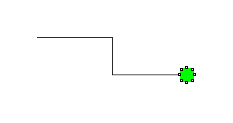
\includegraphics[width=0.4\textwidth]{turtle_example}
    \caption[Example output of turtle--graphics]{Example output of turtle--graphics.}
    \label{fig:turtle_example}
\end{figure}

\subsection{Parameter passing by value and by reference}

In the ImageJ Macro Language parameters that have a basic type, i.e. numbers and strings are passed by value and arrays by reference. This means that when you call {\tt factorial(n)} with a variable $n$ defined in the outer scope, the value of this variable will not be modified. However when you pass a variable containing an array into a function and the function modifies the elements of the array the elements of the array in the outer variable are modified. This is why the output of Listing \ref{lst:call_by_value} is ''5 25'' and the output of Listing \ref{lst:call_by_reference} is ''1, 4, 9'' for $a$ and for $b$.  

\begin{listing}[H]
\begin{minted}[frame=lines, linenos]{java} 
a = 5;
b = squareValue(a);
print(a, b);
function squareValue(a) {
	a = a * a;
	return a;
}
\end{minted}
\caption{The output is ''5 25''; The $a$ in the outer context is not modified by the commands in the function.}
\label{lst:call_by_value} 
\end{listing}

\begin{listing}[H]
\begin{minted}[frame=lines, linenos]{java} 
a = newArray(1,2,3);
b = squareList(a);
Array.print(a);
Array.print(b);

function squareList(a) {
	for (i=0; i<a.length; i++)
		a[i] = a[i] * a[i];
	return a;
}
\end{minted}
\caption{The output is two times ''1, 4, 9''; The $a$ in the outer context is modified by the commands in the function.}
\label{lst:call_by_reference} 
\end{listing}



